\chapter{Appendix of Images} \label{ch:appendix_visual}


\begin{figure}[!ht]
    \fcapside[\FBwidth]{%
        \captionsetup{parskip = .5\baselineskip plus 1pt}%
        \caption[]{%
             Power Delay Profile (PDP) utilized for discrete channel modeling.
        }%
        \label{fig:ch2_pdp}%
    }{%
        
\includegraphics[width=0.40\textwidth]{figures/chap3_channel/1.png}
    }
\end{figure}

\section{Channel 1}

\begin{figure}[!ht]
    \centering
    \captionsetup{parskip = .5\baselineskip plus 1pt}
    \begin{tabular}{ccc}
        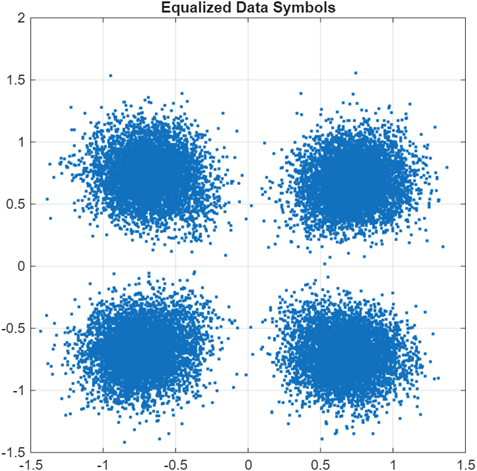
\includegraphics[width=0.3\textwidth]{figures/chap3_channel/c1_3.png} &
        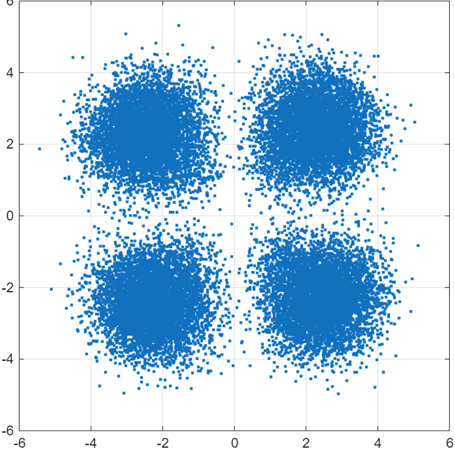
\includegraphics[width=0.3\textwidth]{figures/chap3_channel/c1_4.png} &
        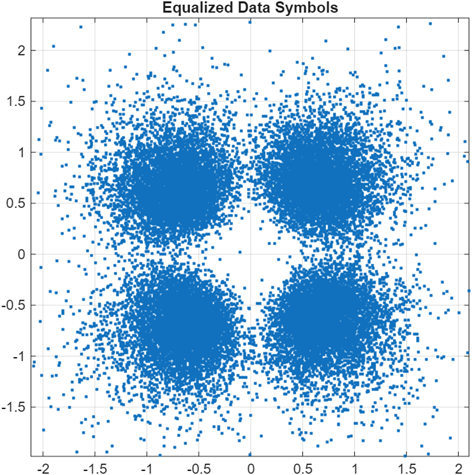
\includegraphics[width=0.3\textwidth]{figures/chap3_channel/c1_2.png} \\
        \small (a) MMSE Equalization & \small (b) LS Equalization & \small (c) No Equalization
    \end{tabular}
    \caption[Channel 1: Comparison of Equalization Techniques]{%
        Constellation comparison for Channel 1: (a) MMSE equalization provides optimal clustering; 
        (b) LS equalization shows higher noise sensitivity; 
        (c) Unequalized signal exhibiting an open eye pattern due to low ISI levels.
    }%
    \label{fig:ch1_constellation_comparison}%
\end{figure}


\begin{figure}[!ht]
    \ffigbox[\FBwidth]{%
        \begin{tabular}{cc}
            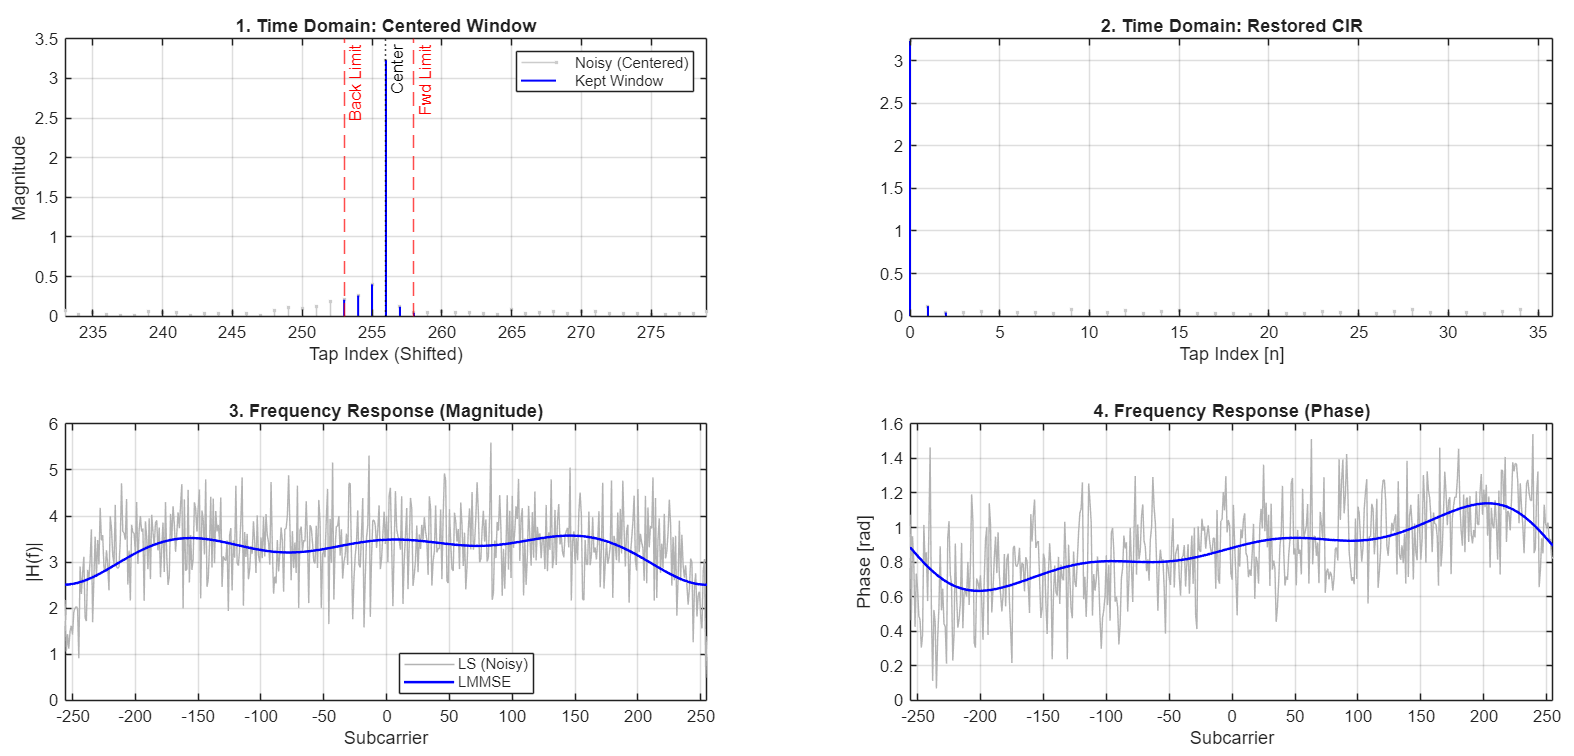
\includegraphics[width=0.67\textwidth]{figures/chap3_channel/c1_1.png} & 
            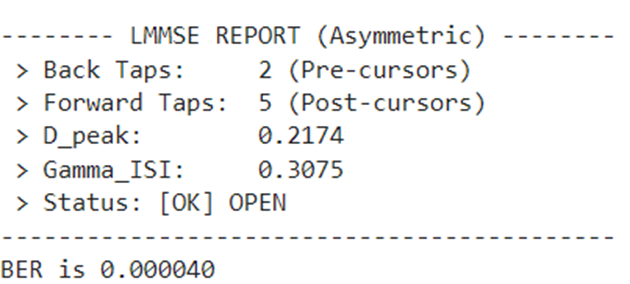
\includegraphics[width=0.27\textwidth]{figures/chap3_channel/c1_5.png} \\
        \end{tabular}
    }{%
        \caption[Channel 1: Estimation and ISI Report]{%
            (Left) Time domain CIR windowing and Frequency Response analysis for Channel 1. 
            (Right) LMMSE numerical report with $\gamma_{\text{ISI}} = 0.3075$, confirming an open eye status ([OK] OPEN).
        }%
        \label{fig:ch1_channel_estimation_summary}%
    }
\end{figure}

\newpage
\section{Channel 2}

\begin{figure}[!ht]
    \centering
    \captionsetup{parskip = .5\baselineskip plus 1pt}
    \begin{tabular}{ccc}
        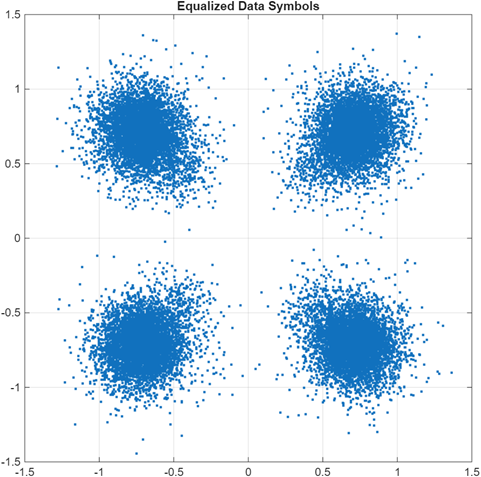
\includegraphics[width=0.3\textwidth]{figures/chap3_channel/c2_2.png} &
        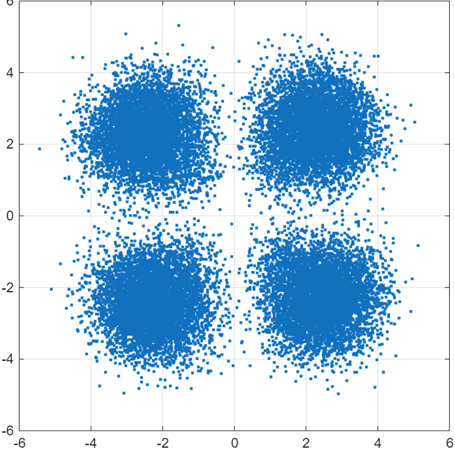
\includegraphics[width=0.3\textwidth]{figures/chap3_channel/c1_4.png} &
        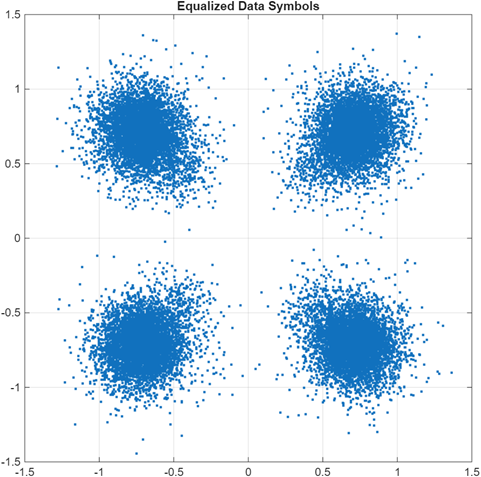
\includegraphics[width=0.3\textwidth]{figures/chap3_channel/c2_2.png} \\
        \small (a) MMSE Equalization & \small (b) LS Equalization & \small (c) No Equalization
    \end{tabular}
    \caption[Channel 2: Equalization Performance]{%
        Comparison of 4-QAM constellations for Channel 2: (a) MMSE equalization effectively minimizes clustering spread; 
        (b) LS equalization displays characteristic noise enhancement; 
        (c) Unequalized signal showing an open eye status due to low intrinsic distortion.
    }%
    \label{fig:ch2_constellations}%
\end{figure}


\begin{figure}[!ht]
    \ffigbox[\FBwidth]{%
        \begin{tabular}{cc}
            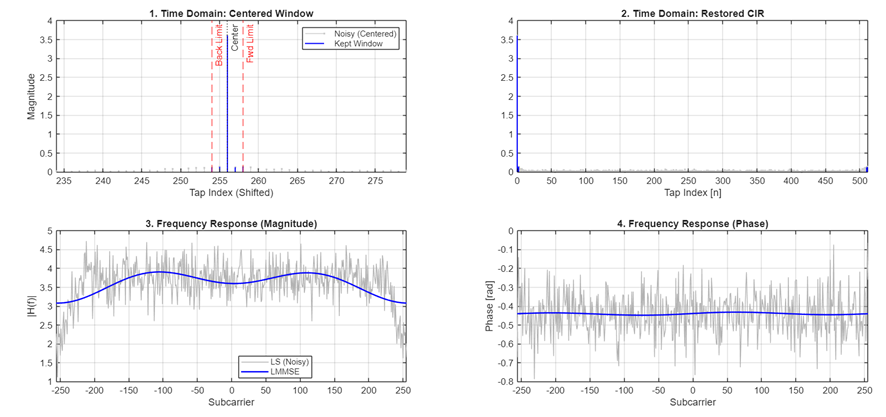
\includegraphics[width=0.67\textwidth]{figures/chap3_channel/c2_1.png} & 
            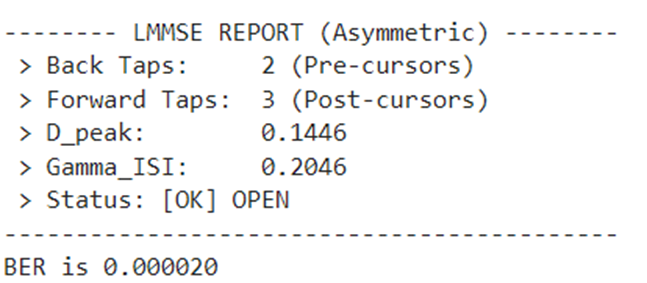
\includegraphics[width=0.27\textwidth]{figures/chap3_channel/c2_3.png} \\
        \end{tabular}
    }{%
        \caption[Channel 2: Response and ISI Report]{%
            (Left) Time domain CIR windowing and Frequency Response magnitude for Channel 2. 
            (Right) LMMSE numerical report indicating $\gamma_{\text{ISI}} = 0.2046$ with an [OK] OPEN status.
        }%
        \label{fig:ch2_report}%
    }
\end{figure}

\newpage
\section{Channel 3}
\begin{figure}[!ht]
    \centering
    \captionsetup{parskip = .5\baselineskip plus 1pt}
    \begin{tabular}{ccc}
        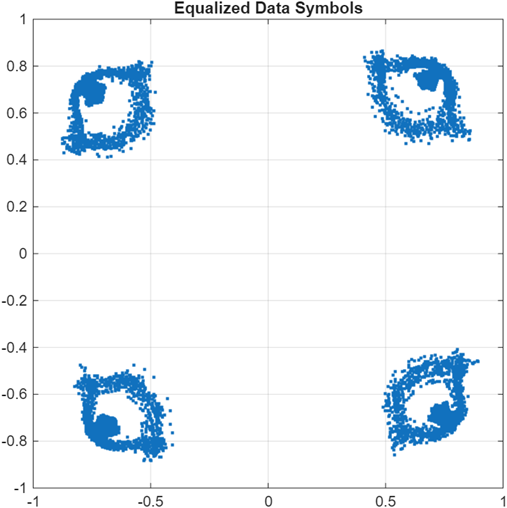
\includegraphics[width=0.3\textwidth]{figures/chap3_channel/c3_3.png} &
        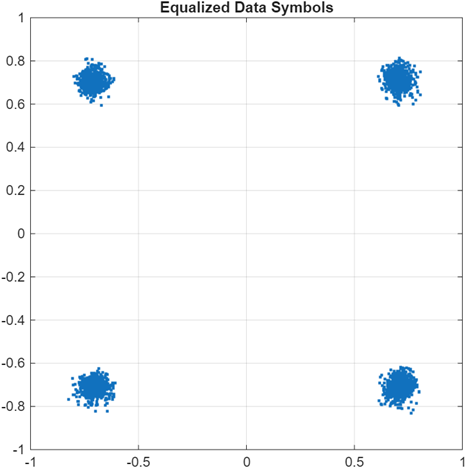
\includegraphics[width=0.3\textwidth]{figures/chap3_channel/c3_4.png} &
        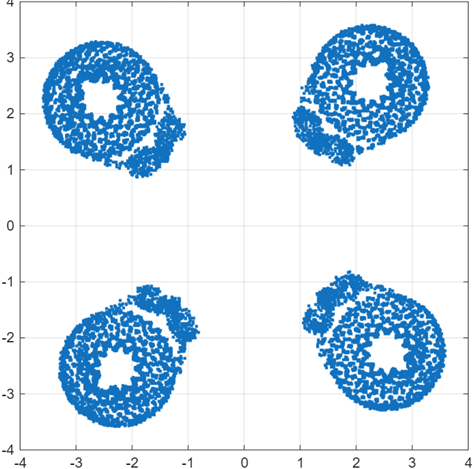
\includegraphics[width=0.3\textwidth]{figures/chap3_channel/c3_5.png} \\
        \small (a) MMSE Equalization & \small (b) LS Equalization & \small (c) No Equalization
    \end{tabular}
    \caption[Comparison of Equalization Techniques]{%
        Constellation comparison: (a) MMSE equalization provides optimal clustering; 
        (b) LS equalization shows higher noise sensitivity; 
        (c) Unequalized signal with a closed eye pattern due to severe ISI.
    }%
    \label{fig:constellation_comparison}%
\end{figure}



\begin{figure}[!ht]
    \ffigbox[\FBwidth]{%
        \begin{tabular}{cc}
            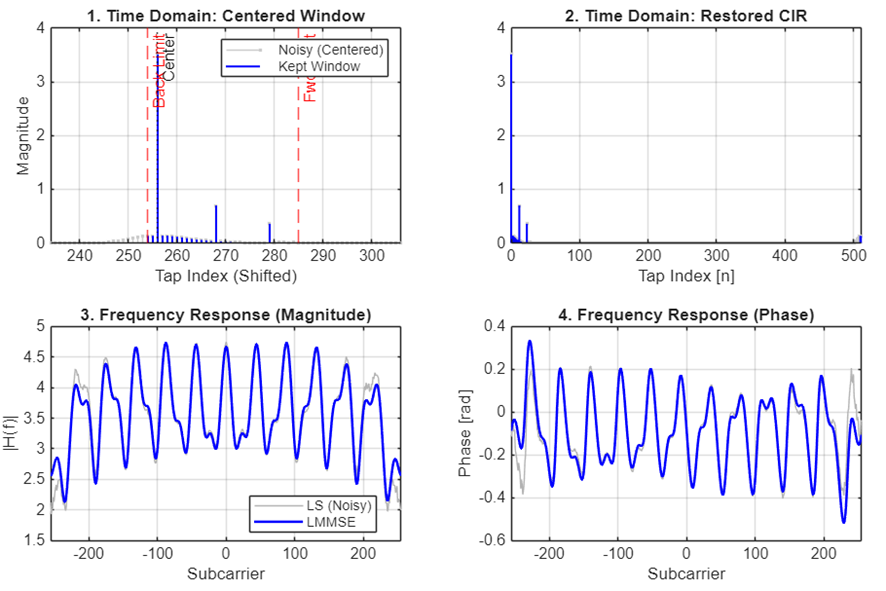
\includegraphics[width=0.67\textwidth]{figures/chap3_channel/c3_1.png} & 
            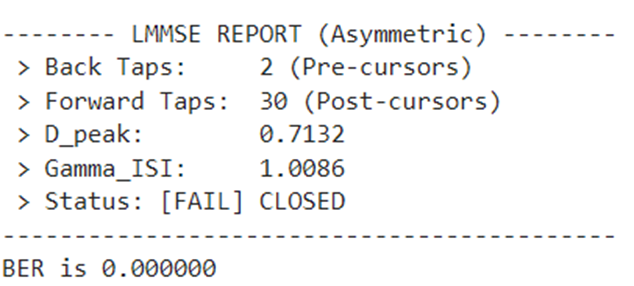
\includegraphics[width=0.27\textwidth]{figures/chap3_channel/c3_2.png} \\
        \end{tabular}
    }{%
        \caption[Channel Estimation and ISI Report]{%
            (Left) Time domain CIR windowing and Frequency Response analysis. 
            (Right) LMMSE numerical report with $\gamma_{\text{ISI}} = 1.0086$, confirming a closed eye status.
        }%
        \label{fig:channel_estimation_summary}%
    }
\end{figure}



\begin{figure}[!ht]
    \fcapside[\FBwidth]{%
        \captionsetup{parskip = .5\baselineskip plus 1pt}%
        \caption[]{%
            Channel Power Delay Profile (PDP).
        }%
        \label{fig:isi-dispersion}%
    }{%
        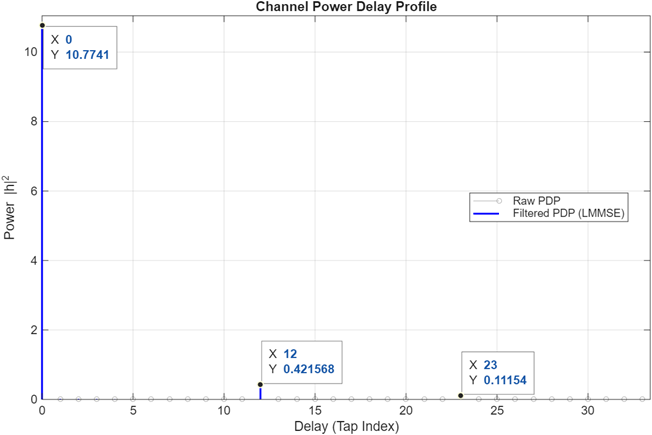
\includegraphics[width=0.60\textwidth]{figures/chap3_channel/c3_6.png}
    }
\end{figure}


\newpage
\section{Channel 4}
\begin{figure}[!ht]
    \centering
    \captionsetup{parskip = .5\baselineskip plus 1pt}
    \begin{tabular}{cc}
        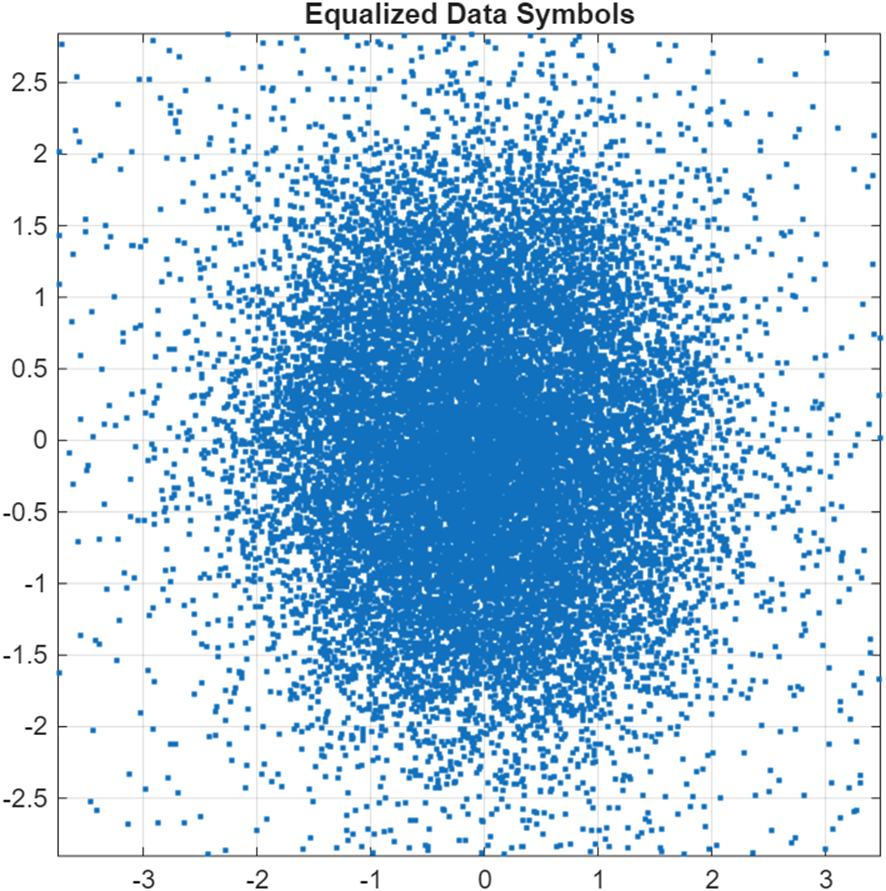
\includegraphics[width=0.45\textwidth]{figures/chap3_channel/c4_1.png} &
        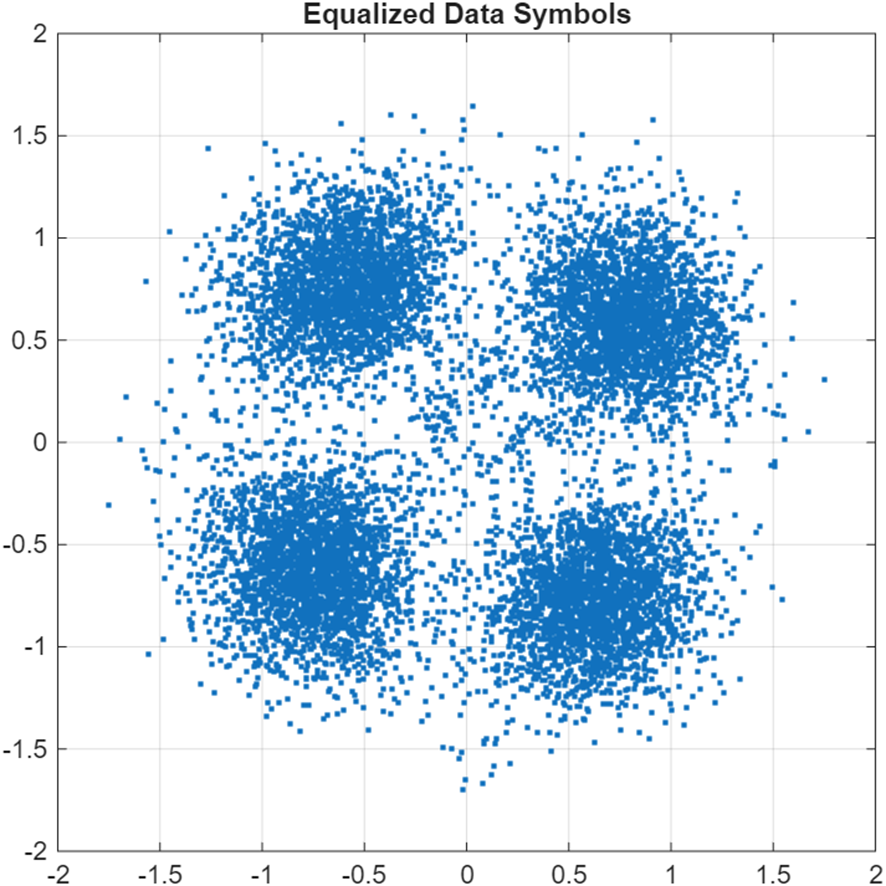
\includegraphics[width=0.45\textwidth]{figures/chap3_channel/c4_3.png} \\
        \small (a) Initial Equalized Symbols & \small (b) Improved Sideband Reception
    \end{tabular}
    \caption[Channel 4: Band-Rejection Equalization Comparison]{%
        Comparison of received 4-QAM constellations for Channel 4: (a) High BER reception due to band-rejection characteristics; 
        (b) Improved constellation achieved by activating sideband subcarriers, leading to lower bit error rates.
    }%
    \label{fig:ch4_constellations}%
\end{figure}


\begin{figure}[!ht]
    \ffigbox[\FBwidth]{%
        \begin{tabular}{cc}
            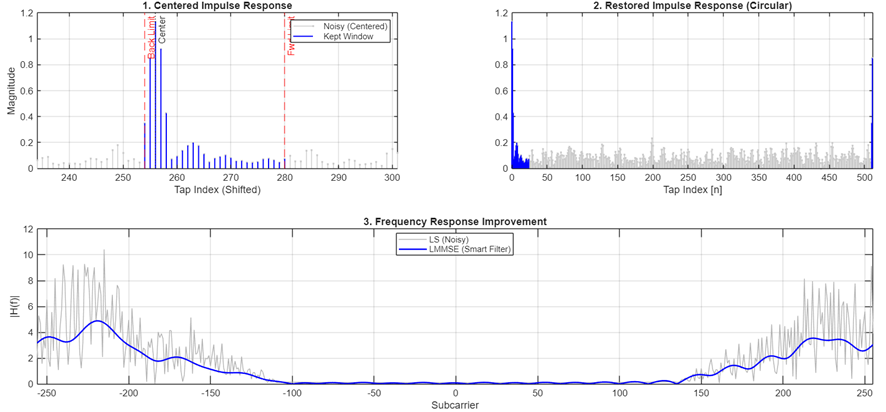
\includegraphics[width=0.67\textwidth]{figures/chap3_channel/c4_6.png} & 
            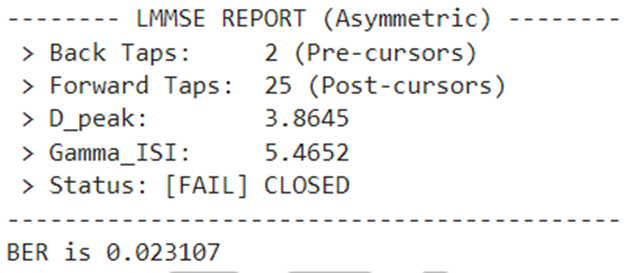
\includegraphics[width=0.27\textwidth]{figures/chap3_channel/c4_4.png} \\
        \end{tabular}
    }{%
        \caption[Channel 4: Frequency Response and Improved Report]{%
            (Left) Frequency response analysis revealing a significant band-rejection notch in the central subcarriers. 
            (Right) Improved LMMSE report for sideband transmission, showing an optimized status despite a high $\gamma_{\text{ISI}} = 5.4652$.
        }%
        \label{fig:ch4_frequency_report}%
    }
\end{figure}


\begin{figure}[!ht]
    \fcapside[\FBwidth]{%
        \captionsetup{parskip = .5\baselineskip plus 1pt}%
        \caption[]{%
            Signal magnitude and normalized correlation metric for Channel 4 frame detection.
        }%
        \label{fig:ch4_correlation}%
    }{%
        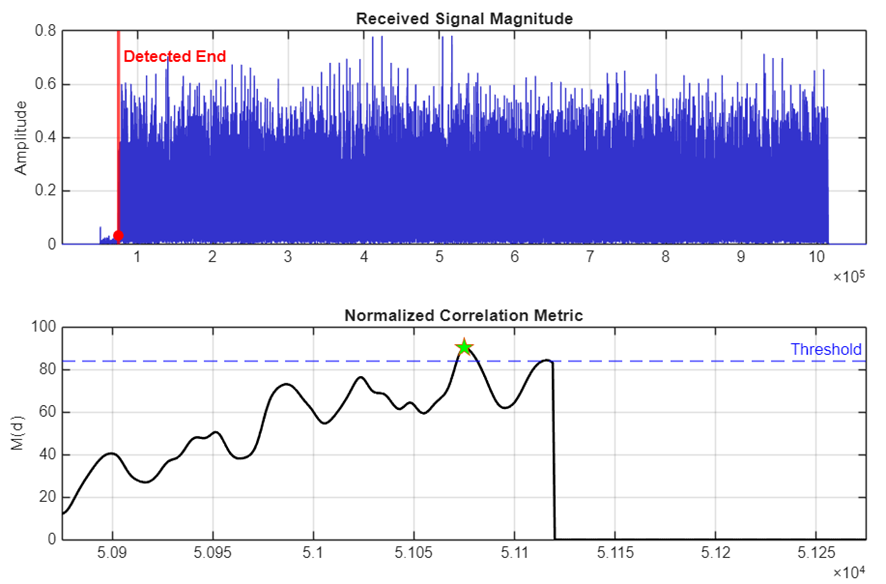
\includegraphics[width=0.60\textwidth]{figures/chap3_channel/c4_5.png}
    }
\end{figure}



\newpage
\section{Channel 5}

\begin{figure}[!ht]
    \fcapside[\FBwidth]{%
        \captionsetup{parskip = .5\baselineskip plus 1pt}%
        \caption[Channel 5: MMSE Equalized Symbols]{%
            Recovered 4-QAM constellation for Channel 5 utilizing LMMSE equalization to mitigate severe ISI.
        }%
        \label{fig:ch5_constellation}%
    }{%
        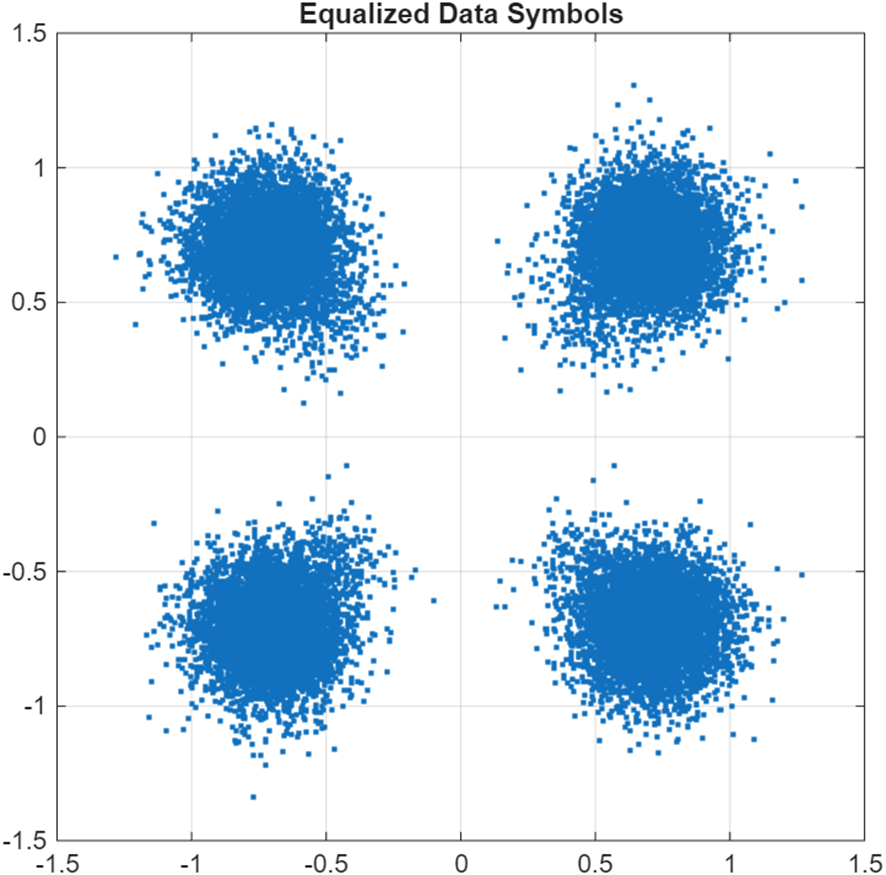
\includegraphics[width=0.60\textwidth]{figures/chap3_channel/c5_1.png}
    }
\end{figure}

\begin{figure}[!ht]
    \centering
    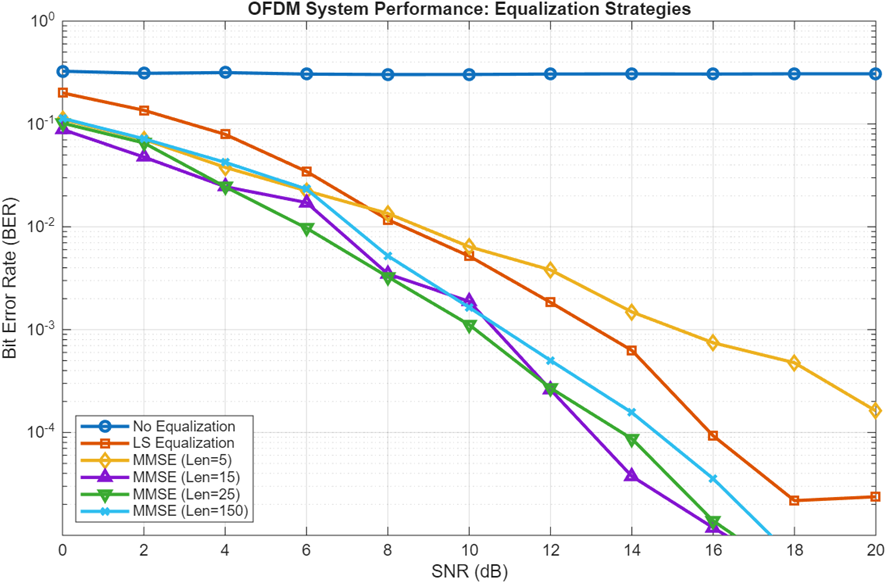
\includegraphics[width=0.85\textwidth]{figures/chap3_channel/c5_2.png}
    \caption[Channel 5: BER Performance Comparison]{%
        Bit Error Rate (BER) performance curves for Channel 5. The plot compares the performance of an unequalized system, LS equalization, and MMSE equalization with varying filter lengths ($L=5, 15, 25, 150$).
    }%
    \label{fig:ch5_ber_performance}%
\end{figure}

\begin{figure}[!ht]
    \ffigbox[\FBwidth]{%
        \begin{tabular}{cc}
            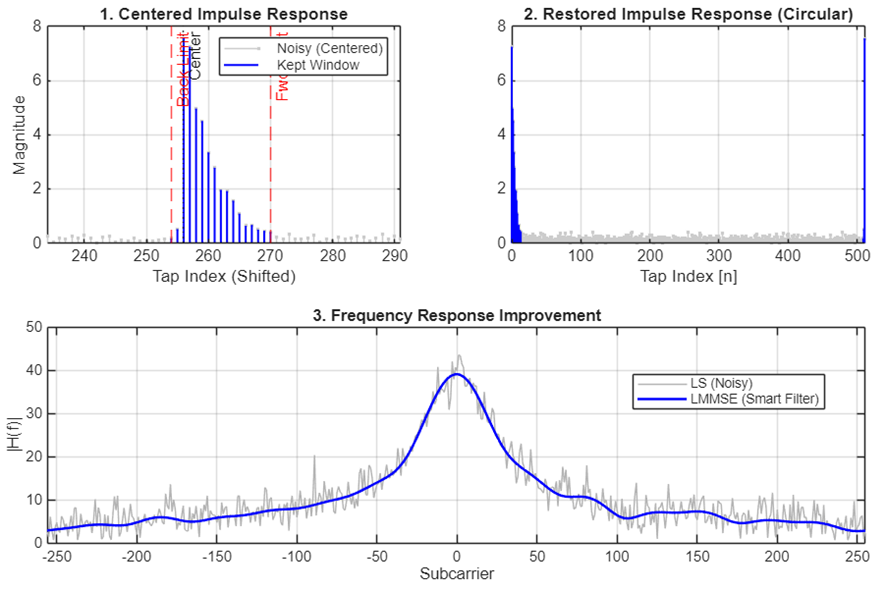
\includegraphics[width=0.67\textwidth]{figures/chap3_channel/c5_3.png} & 
            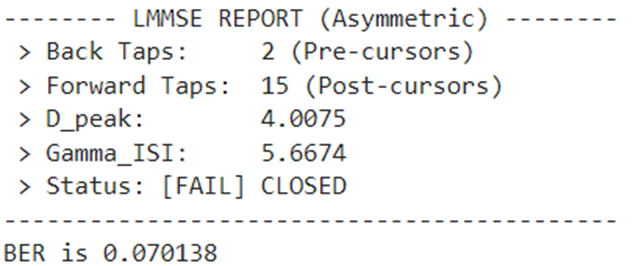
\includegraphics[width=0.27\textwidth]{figures/chap3_channel/c5_4.png} \\
        \end{tabular}
    }{%
        \caption[Channel 5: Estimation and Numerical Report]{%
            (Left) Time-domain CIR and Frequency Response improvement analysis. 
            (Right) LMMSE numerical report showing the critical ISI level $\gamma_{\text{ISI}} = 5.6674$ and a [FAIL] CLOSED status.
        }%
        \label{fig:ch5_numerical_summary}%
    }
\end{figure}

\begin{figure}[!ht]
    \fcapside[\FBwidth]{%
        \captionsetup{parskip = .5\baselineskip plus 1pt}%
        \caption[]{%
            Channel 5 Power Delay Profile (PDP) comparing raw energy and filtered LMMSE distribution.
        }%
        \label{fig:ch5_pdp_analysis}%
    }{%
        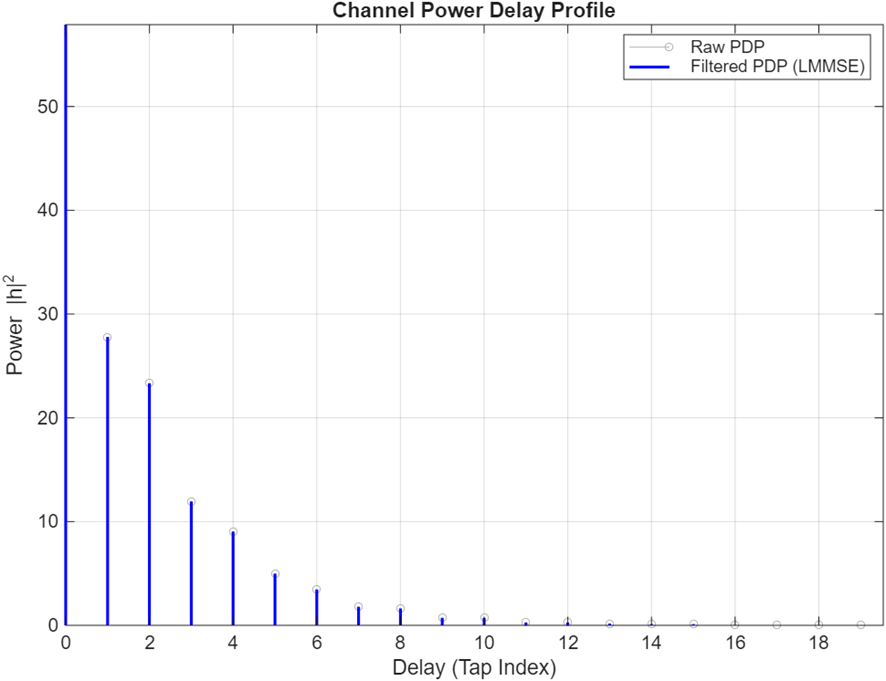
\includegraphics[width=0.60\textwidth]{figures/chap3_channel/c5_5.png}
    }
\end{figure}


%%%%%%%%%%%%%%%%%%%%%%%%%%%%%%%%%%%%%%%%%%%%%%%%%%%%%%%%%%%%%%%
%%%%%%%%%%%%%%%%%%%%%%%%%%%%%%%%%%%%%%%%%%%%%%%%%%%%%%%%%%%%%%%
%%%%%%%%%%%%%%%%%%%%%%%%%%%%%%%%%%%%%%%%%%%%%%%%%%%%%%%%%%%%%%%

\newpage
\section{Transmission Experiments} \label{sec:appendix_transmission}

\begin{figure}[!ht]
    \centering
    \captionsetup{parskip = .5\baselineskip plus 1pt}
    \begin{tabular}{cc}
        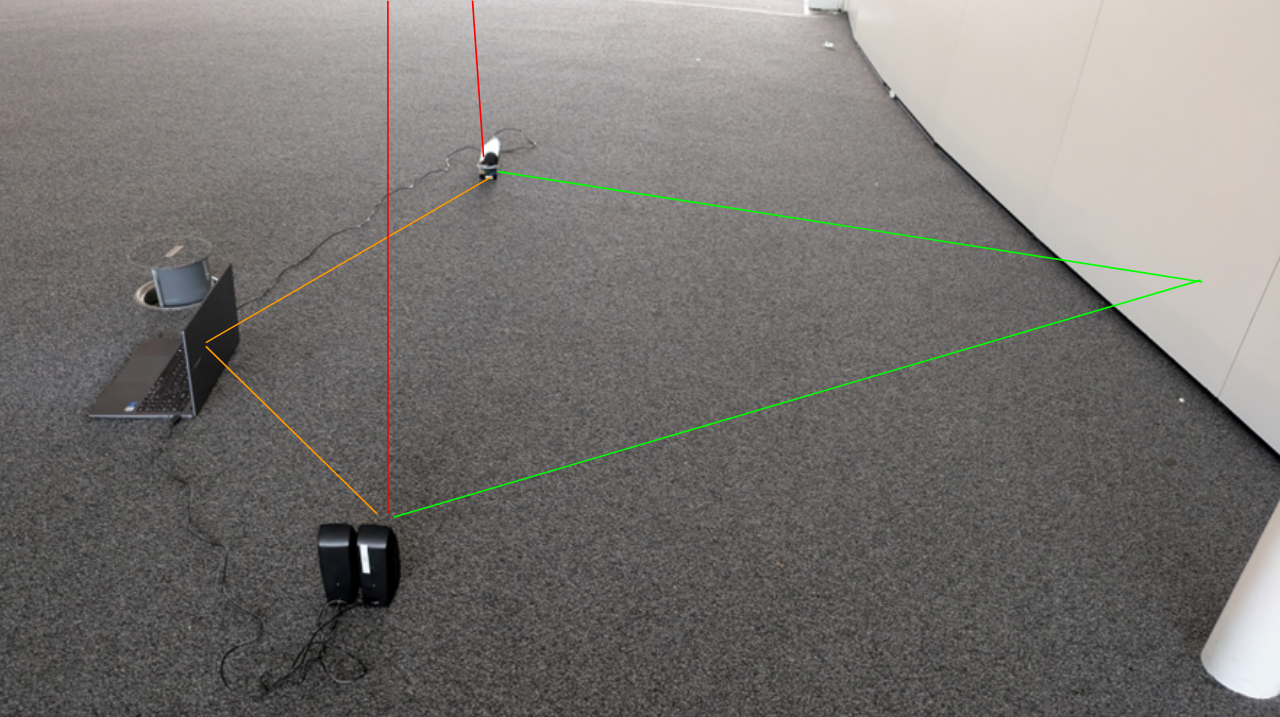
\includegraphics[width=0.47\textwidth]{figures/chap5_transmission/imag1.png} &
        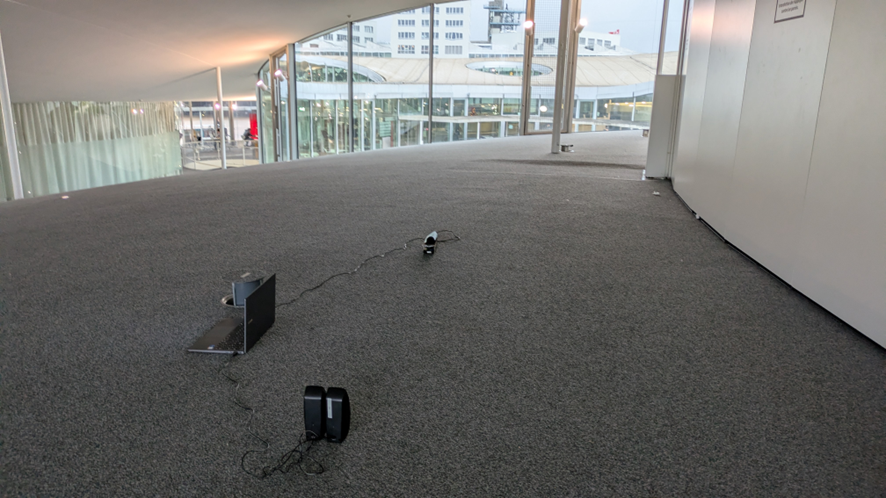
\includegraphics[width=0.47\textwidth]{figures/chap5_transmission/imag2.png} \\
        \small (a) Tx/Rx Setup & \small (b) Environment View
    \end{tabular}
    \caption[Experimental Setup]{%
        Physical experimental setup showing the acoustic transmission environment.
        (a) Relative positioning of the laptop (transmitter/receiver processing) and speakers.
        (b) Wide view of the room characterized by carpeted flooring and glass walls.
    }%
    \label{fig:trans_setup}%
\end{figure}

\begin{figure}[!ht]
    \ffigbox[\FBwidth]{%
        \begin{tabular}{cc}
            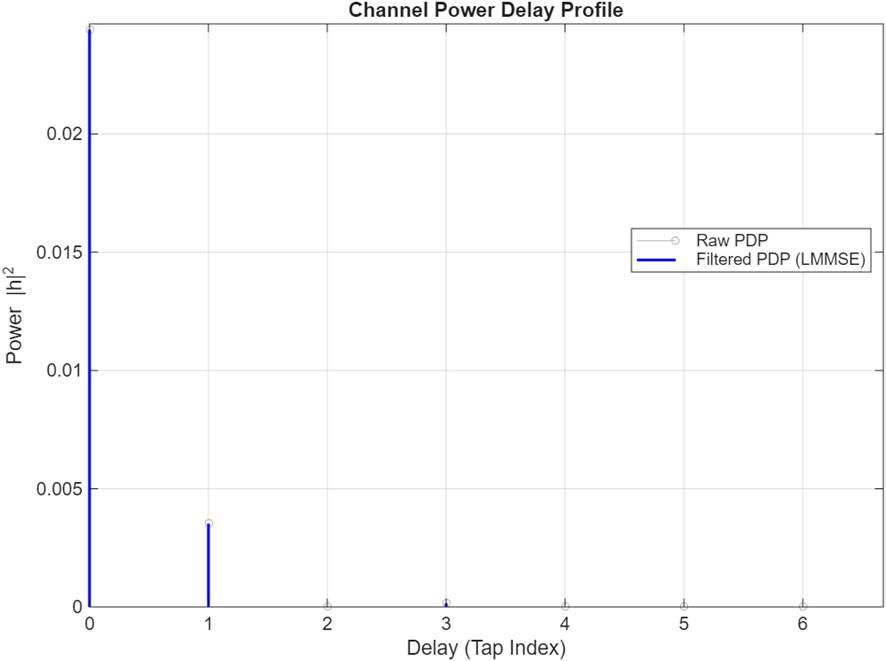
\includegraphics[width=0.48\textwidth]{figures/chap5_transmission/imag6.png} & 
            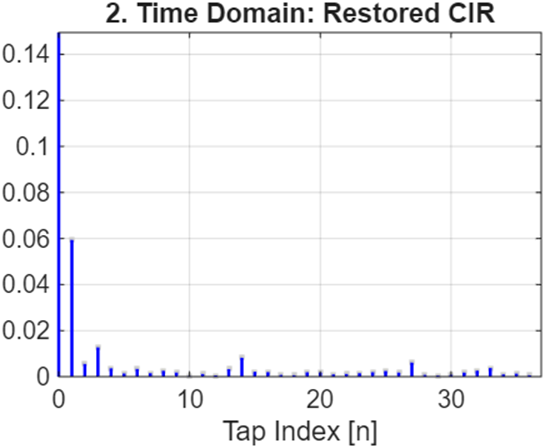
\includegraphics[width=0.45\textwidth]{figures/chap5_transmission/imag7.png} \\
        \end{tabular}
    }{%
        \caption[Channel Impulse Analysis]{%
            (Left) Channel Power Delay Profile (PDP) showing the main path and multipath components. 
            (Right) Restored Time Domain Channel Impulse Response (CIR) used for equalization.
        }%
        \label{fig:trans_cir_pdp}%
    }
\end{figure}

\begin{figure}[!ht]
    \ffigbox[\FBwidth]{%
        \begin{tabular}{cc}
            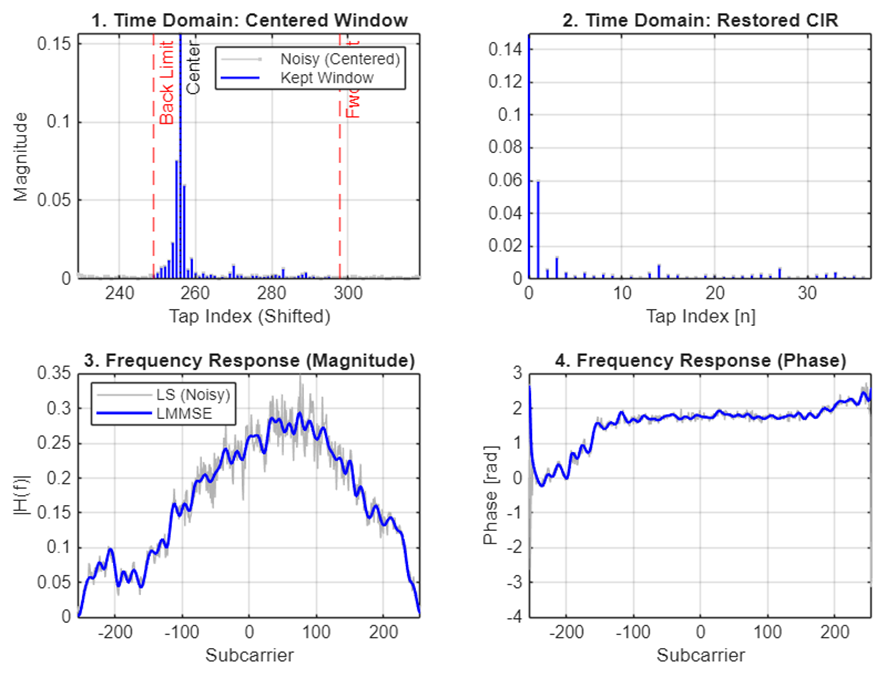
\includegraphics[width=0.64\textwidth]{figures/chap5_transmission/imag4.png} & 
            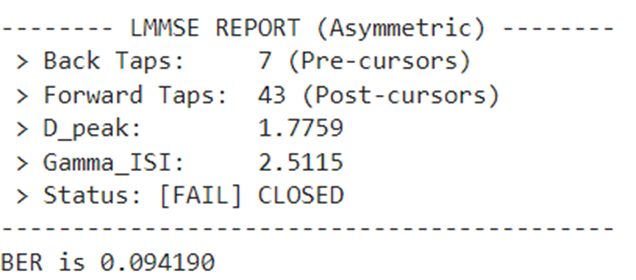
\includegraphics[width=0.29\textwidth]{figures/chap5_transmission/imag8.png} \\
        \end{tabular}
    }{%
        \caption[LMMSE Estimation Report]{%
            (Left) Detailed channel estimation plots: windowing strategy, CIR, and frequency response (magnitude and phase). 
            (Right) LMMSE numerical report showing estimation parameters, $\gamma_{\text{ISI}} = 2.5115$, and a resulting BER of \num{0.094190}.
        }%
        \label{fig:trans_lmmse_report}%
    }
\end{figure}

\begin{figure}[!ht]
    \fcapside[\FBwidth]{%
        \captionsetup{parskip = .5\baselineskip plus 1pt}%
        \caption[Image Transmission Result]{%
            Visual comparison between the original transmitted test pattern and the received image after equalization and decoding, illustrating the impact of the acoustic channel.
        }%
        \label{fig:trans_image_result}%
    }{%
        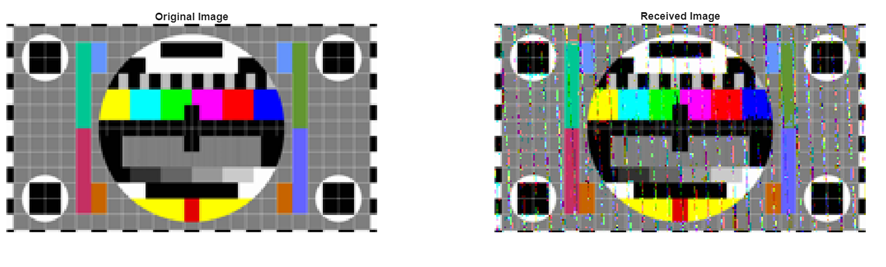
\includegraphics[width=0.75\textwidth]{figures/chap5_transmission/imag5.png}
    }
\end{figure}